\usepackage{tikz}

\newcommand {\Lysine}[1] {
	\begin{scope}[scale=0.5]	% Lysine
	\path (#1) node (zero) {};
	\draw[to_2]  (zero.center)	-- ++(30:1) node (CO) {}
	        -- +(330:1) node [anchor=base] {O$^{\mbox{-}}$};
	\draw[to_1]  (CO.center) 	-- +(90:1) node (Od) {O};
	\draw[to_1i] (CO.30)		-- +(90:1);
	\draw[to_3]  (zero.center)	-- ++(150:1) node {NH$_{\mbox{3}}^{\mbox{+}}$};
	\draw[to_3]  (zero.center)	-- ++(270:1) node(Cb){}
	        -- ++(330:1) node (Cc) {}
	        -- ++(270:1) node (Cd) {}
	        -- ++(210:1) node (Ce) {}
	        -- ++(150:1) node (Cf) {NH$_{\mbox{2}}$};
	\end{scope}
}
\newcommand{\Asparagine}[1]{
	\begin{scope}[scale=0.5]	% Asparagine
	\path (#1) node (zero) {};
	\draw[to_2]  (zero.center)	-- ++(30:1) node (CO) {}
	        -- +(330:1) node [anchor=base] {O$^{\mbox{-}}$};
	\draw[to_1]  (CO.center)	-- +(90:1) node (Od) {O};
	\draw[to_1i] (CO.30)		-- +(90:1);
	\draw[to_3]  (zero.center)	-- ++(150:1) node {NH$_{\mbox{3}}^{\mbox{+}}$};
	\draw[to_2]  (zero.center)	-- ++(270:1) node(Cb){}
	        -- ++(330:1) node (Cc) {}
	        -- +(30:1) node (Cd) {NH$_{\mbox{2}}$};
	\draw[to_1i] (Cc.center)	-- +(270:1) node (O) {};
	\draw[to_1]  (Cc.210)		-- (O.150);
	\path (O.center) node {O};
	\end{scope}
}

\newcommand{\Arginine}[1]{
	\begin{scope}[scale=0.5]	% \Arginine
	\path (#1) node (zero) {};
	\draw[to_2]  (zero.center)	-- ++(30:1) node (CO) {}
	        -- +(330:1) node [anchor=base] {O$^{\mbox{-}}$};
	\draw[to_1]  (CO.center)	-- +(90:1) node (Od) {O};
	\draw[to_1i] (CO.30)		-- +(90:1);
	\draw[to_3]  (zero.center)	-- ++(150:1) node {NH$_{\mbox{3}}^{\mbox{+}}$};
	\draw[to_2]  (zero.center)	-- ++(270:1) node(Cb){}
	        -- ++(330:1) node (Cc) {}
	        -- ++(270:1) node (Cd) {}
	        -- ++(330:1) node (NH1) {NH};
	\draw[from_2,to_3]  (NH1.center)	-- ++(30:1) node (Ce) {}
	        -- ++(330:1) node {NH$_{\mbox{2}}$};
	\draw[to_1i] (Ce.center)	-- ++(90:1) node (N2) {};
	\draw[to_1]  (Ce.150)		-- (N2.210);
	\path (N2) node {N};
	\end{scope}
}

\newcommand{\Serine}[1]{
	\begin{scope}[scale=0.5]	% Serine
	\path (#1) node (zero) {};
	\draw[to_2]  (zero.center)	-- ++(30:1) node (CO) {}
	        -- +(330:1) node [anchor=base] {O$^{\mbox{-}}$};
	\draw[to_1]  (CO.center)	-- +(90:1) node (Od) {O};
	\draw[to_1i] (CO.30)		-- +(90:1);
	\draw[to_3]  (zero.center)	-- ++(150:1) node {NH$_{\mbox{3}}^{\mbox{+}}$};
	\draw[to_2]  (zero.center)	-- ++(270:1) node(Cb){} -- ++(210:1) node (Cc) {OH};
	\end{scope}
}

\newcommand{\Threonine}[1]{
	\begin{scope}[scale=0.5]	% Threonine
	\path (#1) node (zero) {};
	\draw[to_2]  (zero.center)	-- ++(30:1) node (CO) {}
	        -- +(330:1) node [anchor=base] {O$^{\mbox{-}}$};
	\draw[to_1]  (CO.center)	-- +(90:1) node (Od) {O};
	\draw[to_1i] (CO.30)		-- +(90:1);
	\draw[to_3]  (zero.center)	-- ++(150:1) node {NH$_{\mbox{3}}^{\mbox{+}}$};
	\draw[to_2]  (zero.center)	-- ++(270:1) node(Cb){}
	        -- ++(330:1) node (Cc) {} (Cb.center)
	        -- +(210:1) node {OH};
	\end{scope}
}
\newcommand{\Methionine}[1]{
\begin{scope}[scale=0.5]	% Methionine
\path (#1) node (zero) {};
\draw[to_2]  (zero.center)	-- ++(30:1) node (CO) {}
        -- +(330:1) node [anchor=base] {O$^{\mbox{-}}$};
\draw[to_1]  (CO.center)	-- +(90:1) node (Od) {O};
\draw[to_1i] (CO.30)		-- +(90:1);
\draw[to_3]  (zero.center)	-- ++(150:1) node {NH$_{\mbox{3}}^{\mbox{+}}$};
\draw[to_1]  (zero.center)	-- ++(270:1) node(Cb){}
        -- ++(330:1) node (Cc) {}
        -- ++(30:1) node (Cd) {S};
\draw[from_1] (Cd.center)	-- +(330:1);
\end{scope}
}
\newcommand{\Isoleucine}[1]{
	\begin{scope}[scale=0.5]	% Isoleucine
	\path (#1) node (zero) {};
	\draw[to_2]  (zero.center)	-- ++(30:1) node (CO) {}
	        -- +(330:1) node [anchor=base] {O$^{\mbox{-}}$};
	\draw[to_1]  (CO.center)	-- +(90:1) node (Od) {O};
	\draw[to_1i] (CO.30)		-- +(90:1);
	\draw[to_3]  (zero.center)	-- ++(150:1) node {NH$_{\mbox{3}}^{\mbox{+}}$};
	\draw	     (zero.center)	-- ++(270:1) node(Cb){}
	        -- ++(330:1) node (Cc) {}
	        -- +(30:1) node (Cd) {} (Cb.center)
	        -- +(210:1) node (Ce) {};
	\end{scope}
}

\newcommand{\GlutamicAcid}[1]{
\begin{scope}[scale=0.5]	% Glutamic acid
	\path (#1) node (zero) {};
	\draw[to_2]  (zero.center)	-- ++(30:1) node (CO) {}
	        -- +(330:1) node [anchor=base] {O$^{\mbox{-}}$};
	\draw[to_1]  (CO.center)  	-- +(90:1) node (Od) {O};
	\draw[to_1i] (CO.30)  		-- +(90:1);
	\draw[to_3]  (zero.center) 	-- ++(150:1) node {NH$_{\mbox{3}}^{\mbox{+}}$};
	\draw[to_1i] (zero.center) 	-- ++(270:1) node(Cb){}
	        -- ++(330:1) node (Cc) {}
	        -- ++(270:1) node (Cd) {}
	        -- ++(330:1) node (NH) {OH};
	\draw[to_1]  (Cd.center) 	-- +(210:1) node (O) {};
	\draw[to_1i] (Cd.270) 		-- (O.300);
	\path (O.center) node {O};
	\end{scope}
}
\newcommand{\AsparticAcid}[1]{
	\begin{scope}[scale=0.5]	% Aspartic acid
	\path (#1) node (zero) {};
	\draw[to_2]  (zero.center)	-- ++(30:1) node (CO) {}
	        -- +(330:1) node [anchor=base] {O$^{\mbox{-}}$};
	\draw[to_1]  (CO.center) 	-- +(90:1) node (Od) {O};
	\draw[to_1i] (CO.30)		-- +(90:1);
	\draw[to_3]  (zero.center)	-- ++(150:1) node {NH$_{\mbox{3}}^{\mbox{+}}$};
	\draw[to_2]  (zero.center)	-- ++(270:1) node(Cb){}
	        -- ++(330:1) node (Cc) {}
	        -- +(30:1) node (Cd) {OH};
	\draw[to_1i] (Cc.center)	-- +(270:1) node (O) {};
	\draw[to_1]  (Cc.210)		-- (O.150);
	\path (O.center) node {O};
	\end{scope}
}
\newcommand{\Glycine}[1]{
	\begin{scope}[scale=0.5]	% Glycine
	\path (#1) node (zero) {};
	\draw[to_2]  (zero.center)	-- ++(30:1) node (CO) {}
	        -- +(330:1) node [anchor=base] {O$^{\mbox{-}}$};
	\draw[to_1]  (CO.center)	-- +(90:1) node (Od) {O};
	\draw[to_1i] (CO.30)		-- +(90:1);
	\draw[to_3]  (zero.center)	-- ++(150:1) node {NH$_{\mbox{3}}^{\mbox{+}}$};
	\end{scope}
}

\newcommand{\Alanine}[1]{
	\begin{scope}[scale=0.5]	% Alanine
	\path (#1) node (zero) {};
	\draw[to_2]  (zero.center)	-- ++(30:1) node (CO) {}
	        -- +(330:1) node [anchor=base] {O$^{\mbox{-}}$};
	\draw[to_1]  (CO.center)	-- +(90:1) node (Od) {O};
	\draw[to_1i] (CO.30)		-- +(90:1);
	\draw[to_3]  (zero.center)	-- ++(150:1) node {NH$_{\mbox{3}}^{\mbox{+}}$};
	\draw	     (zero.center)	-- ++(270:1) node(Cb){};
	\end{scope}
}
\newcommand{\Valine}[1]{
	\begin{scope}[scale=0.5]	% Valine
	\path (#1) node (zero) {};
	\draw[to_2]  (zero.center)	-- ++(30:1) node (CO) {}
	        -- +(330:1) node [anchor=base] {O$^{\mbox{-}}$};
	\draw[to_1]  (CO.center)	-- +(90:1) node (Od) {O};
	\draw[to_1i] (CO.30)		-- +(90:1);
	\draw[to_3]  (zero.center)	-- ++(150:1) node {NH$_{\mbox{3}}^{\mbox{+}}$};
	\draw (zero.center)		-- ++(270:1) node(Cb){}
	        -- ++(330:1) node (Cc) {};
	\end{scope}
}
\newcommand{\Glutamine}[1]{
	\begin{scope}[scale=0.5]	% Glutamine
	\path (#1) node (zero) {};
	\draw[to_2]  (zero.center)	-- ++(30:1) node (CO) {}
	        -- +(330:1) node [anchor=base] {O$^{\mbox{-}}$};
	\draw[to_1]  (CO.center)	-- +(90:1) node (Od) {O};
	\draw[to_1i] (CO.30)		-- +(90:1);
	\draw[to_2]  (zero.center)	-- ++(150:1) node {NH$_{\mbox{3}}^{\mbox{+}}$};
	\draw[to_3]  (zero.center)	-- ++(270:1) node(Cb){}
	        -- ++(330:1) node (Cc) {}
	        -- ++(270:1) node (Cd) {}
	        -- ++(330:1) node (NH) {NH$_{\mbox{2}}$};
	\draw[to_1]  (Cd.center)	-- +(210:1) node (O) {};
	\draw[to_1i] (Cd.270)		-- (O.300);
	\path (O.center) node {O};
	\end{scope}
}
\newcommand{\Histidine}[1]{
	\begin{scope}[scale=0.5]	% Histidine
	\path (#1) node (zero) {};
	\draw[to_2]  (zero.center)	-- ++(30:1) node (CO) {}
	        -- +(330:1) node [anchor=base] {O$^{\mbox{-}}$};
	\draw[to_1]  (CO.center)	-- +(90:1) node (Od) {O};
	\draw[to_1i] (CO.30)		-- +(90:1);
	\draw[to_3]  (zero.center)	-- ++(150:1) node {NH$_{\mbox{3}}^{\mbox{+}}$};
	\draw        (zero.center)	-- ++(270:1) node(Cb){}
	        -- ++(330:1) node(Cc){};
	\draw[to_2]  (Cc.center)	-- ++(108-1*72:1) node (Cd) {}
	        -- ++(108-2*72:1) node (Ce) {NH};
	\draw[from_1,to_1] (Ce.center)	-- ++(108-3*72:1) node (Cf) {}
	        -- ++(108-4*72:1) node (Cg) {};
	\draw[from_1] (Cg.center)	-- (Cc.center);
	\draw         (Cc.198+2*72)	-- (Cd.198+1*72);
	\draw[from_1] (Cg.72)		-- (Cf.198+4*72);
	\draw (Cg.center) node {N};
	\end{scope}
}

\newcommand{\Proline}[1]{
	\begin{scope}[scale=0.5]	% Proline
	\path (#1) node (zero) {};
	\draw[to_2]  (zero.center)	-- ++(30:1) node (CO) {}
	        -- +(330:1) node [anchor=base] {O$^{\mbox{-}}$};
	\draw[to_1]  (CO.center)	-- +(90:1) node (Od) {O};
	\draw[to_1i] (CO.30)		-- +(90:1);
	\draw[to_2]  (zero.center)	-- ++(150:1) node (nh) {NH$_{\mbox{2}}^+$};
	\draw        (zero.center)	-- ++(270:1) node(Cb){};
	\path        (Cb.center)	-- +(150:1) node (x) {};
	\path        (x.center)  	+(170:1) node (Cd) {};
	\path        (x.center)  	+(250:1) node (Cc) {};
	\draw[to_3]  (Cb.center)	-- (Cc.center)
	        -- (Cd.center)
	        -- (nh.center);
	\end{scope}
}
\newcommand{\Leucine}[1]{
	\begin{scope}[scale=0.5]	% Leucine
	\path (#1) node (zero) {};
	\draw[to_2]  (zero.center)	-- ++(30:1) node (CO) {}
	        -- +(330:1) node [anchor=base] {O$^{\mbox{-}}$};
	\draw[to_1]  (CO.center)	-- +(90:1) node (Od) {O};
	\draw[to_1i] (CO.30)		-- +(90:1);
	\draw[to_3]  (zero.center)	-- ++(150:1) node {NH$_{\mbox{3}}^{\mbox{+}}$};
	\draw (zero.center)		-- ++(270:1) node(Cb){}
	        -- ++(330:1) node (Cc) {}
	        -- +(30:1) node (Cd) {} (Cc.center)
	        -- +(270:1) node (Ce) {};
	\end{scope}
}
\newcommand{\Tyrosine}[1]{
	\begin{scope}[scale=0.5]	% Tyrosine
	\path (#1) node (zero) {};
	\draw[to_2]  (zero.center)	-- ++(30:1) node (CO) {}
	        -- +(330:1) node [anchor=base] {O$^{\mbox{-}}$};
	\draw[to_1]  (CO.center)	-- +(90:1) node (Od) {O};
	\draw[to_1i] (CO.30)		-- +(90:1);
	\draw[to_3]  (zero.center)	-- ++(150:1) node {NH$_{\mbox{3}}^{\mbox{+}}$};
	\draw 	     (zero.center)	-- ++(270:1) node(Cb){};
	\draw	     (Cb.center)	-- ++(330:1) node (Cc) {}
	        -- ++(30:1) node (Cd) {}
	        -- ++(330:1) node (Ce) {}
	        -- ++(270:1) node (Cf) {}
	        -- ++(210:1) node (Cg) {}
	        -- ++(150:1) node (Ch) {}
	        -- ++(90:1);
	\draw        (Cc.330)		-- (Cd.270);
	\draw        (Ce.210)		-- (Cf.150);
	\draw        (Cg.90)		-- (Ch.30);
	\draw[to_1i] (Cf.center)	-- +(330:1) node (OH) {OH};
	\end{scope}
}

\newcommand{\Tryptophane}[1]{
	\begin{scope}[scale=0.5]	% Tryptophane
	\path (#1) node (zero) {};
	\draw[to_2]  (zero.center)	-- ++(30:1) node (CO) {}
	        -- +(330:1) node [anchor=base] {O$^{\mbox{-}}$};
	\draw[to_1]  (CO.center)	-- +(90:1) node (Od) {O};
	\draw[to_1i] (CO.30)		-- +(90:1);
	\draw[to_3]  (zero.center)	-- ++(150:1) node {NH$_{\mbox{3}}^{\mbox{+}}$};
	\draw 	     (zero.center)	-- ++(270:1) node(Cb){}
	        -- ++(330:1) node(Cc){};
	\draw[to_2]  (Cc.center)	-- ++(108-1*72:1) node (Cd) {}
	        -- ++(108-2*72:1) node (Ce) {NH};
	\draw[from_1](Ce.center)	-- ++(108-3*72:1) node (Cf) {}
	        -- ++(108-4*72:1) node (Cg) {};
	\draw 	     (Cg.center)	-- (Cc.center);
	\draw        (Cc.198+2*72)	-- (Cd.198+1*72);
	\draw 	     (Cg.72)		-- (Cf.198+4*72);
	\draw	     (Cg.center)	-- ++(240:1) node (Ch) {}
	        -- ++(300:1) node (Ci) {}
	        -- ++(0:1) node (Cj) {}
	        -- ++(60:1) node (Ck) {}
	        -- ++(120:1) node (Cl) {};
	\draw	     (Ch.0)		-- (Ci.60);
	\draw	     (Cj.120)		-- (Ck.180);
	\end{scope}
}
\newcommand{\Cysteine}[1]{
	\begin{scope}[scale=0.5]	% Cysteine
	\path (#1) node (zero) {};
	\draw[to_2]  (zero.center)	-- ++(30:1) node (CO) {}
	        -- +(330:1) node [anchor=base] {O$^{\mbox{-}}$};
	\draw[to_1]  (CO.center)	-- +(90:1) node (Od) {O};
	\draw[to_1i] (CO.30)		-- +(90:1);
	\draw[to_3]  (zero.center)	-- ++(150:1) node {NH$_{\mbox{3}}^{\mbox{+}}$};
	\draw[to_2]  (zero.center)	-- ++(270:1) node(Cb){}
	        -- ++(210:1) node (Cc) {SH};
	\end{scope}
}

\newcommand{\Selenocysteine}[1]{
	\begin{scope}[scale=0.5]	% Selenocysteine
	\path (#1) node (zero) {};
	\draw[to_2]  (zero.center)	-- ++(30:1) node (CO) {}
	        -- +(330:1) node [anchor=base] {O$^{\mbox{-}}$};
	\draw[to_1]  (CO.center)	-- +(90:1) node (Od) {O};
	\draw[to_1i] (CO.30)		-- +(90:1);
	\draw[to_3]  (zero.center)	-- ++(150:1) node {NH$_{\mbox{3}}^{\mbox{+}}$};
	\draw[to_2]  (zero.center)	-- ++(270:1) node(Cb){}
	        -- ++(210:1) node (Cc) {SeH};
	\end{scope}
}
\newcommand{\SerineT}[1]{
	\begin{scope}[scale=0.5]	% Serine
	\path (#1) node (zero) {};
	\draw[to_2]  (zero.center)	-- ++(30:1) node (CO) {}
	        -- +(330:1) node [anchor=base] {O$^{\mbox{-}}$};
	\draw[to_1]  (CO.center)	-- +(90:1) node (Od) {O};
	\draw[to_1i] (CO.30)		-- +(90:1);
	\draw[to_3]  (zero.center)	-- ++(150:1) node {NH$_{\mbox{3}}^{\mbox{+}}$};
	\draw[to_2]  (zero.center)	-- ++(270:1) node(Cb){}
	        -- ++(330:1) node (Cc) {OH};
	\end{scope}
}
\newcommand{\LeucineT}[1]{
	\begin{scope}[scale=0.5]	% Leucine
	\path (#1) node (zero) {};
	\draw[to_2]  (zero.center)	-- ++(30:1) node (CO) {}
	        -- +(330:1) node [anchor=base] {O$^{\mbox{-}}$};
	\draw[to_1]  (CO.center)	-- +(90:1) node (Od) {O};
	\draw[to_1i] (CO.30)		-- +(90:1);
	\draw[to_3]  (zero.center)	-- ++(150:1) node {NH$_{\mbox{3}}^{\mbox{+}}$};
	\draw 	     (zero.center)	-- ++(270:1) node(Cb){}
	        -- ++(210:1) node (Cc) {}
	        -- +(150:1) node (Cd) {} (Cc.center)
	        -- +(270:1) node (Ce) {};
	\end{scope}
}
\newcommand{\Phenylalanine}[1]{
	\begin{scope}[scale=0.5]	% Phenylalanine
	\path (#1) node (zero) {};
	\draw[to_2]  (zero.center)	-- ++(30:1) node (CO) {}
	        -- +(330:1) node [anchor=base] {O$^{\mbox{-}}$};
	\draw[to_1]  (CO.center)	-- +(90:1) node (Od) {O};
	\draw[to_1i] (CO.30)		-- +(90:1);
	\draw[to_3]  (zero.center)	-- ++(150:1) node {NH$_{\mbox{3}}^{\mbox{+}}$};
	\draw	     (zero.center)	-- ++(270:1) node(Cb){};
	\draw	     (Cb.center)	-- ++(210:1) node (Cc) {}
	        -- ++(150:1) node (Cd) {}
	        -- ++(210:1) node (Ce) {}
	        -- ++(270:1) node (Cf) {}
	        -- ++(330:1) node (Cg) {}
	        -- ++(30:1) node (Ch) {}
	        -- ++(90:1);
	\draw	     (Cc.210)		-- (Cd.270);
	\draw	     (Ce.330)		-- (Cf.30);
	\draw	     (Cg.90)		-- (Ch.150);
	\end{scope}
}

\newcommand{\aapicture}{
	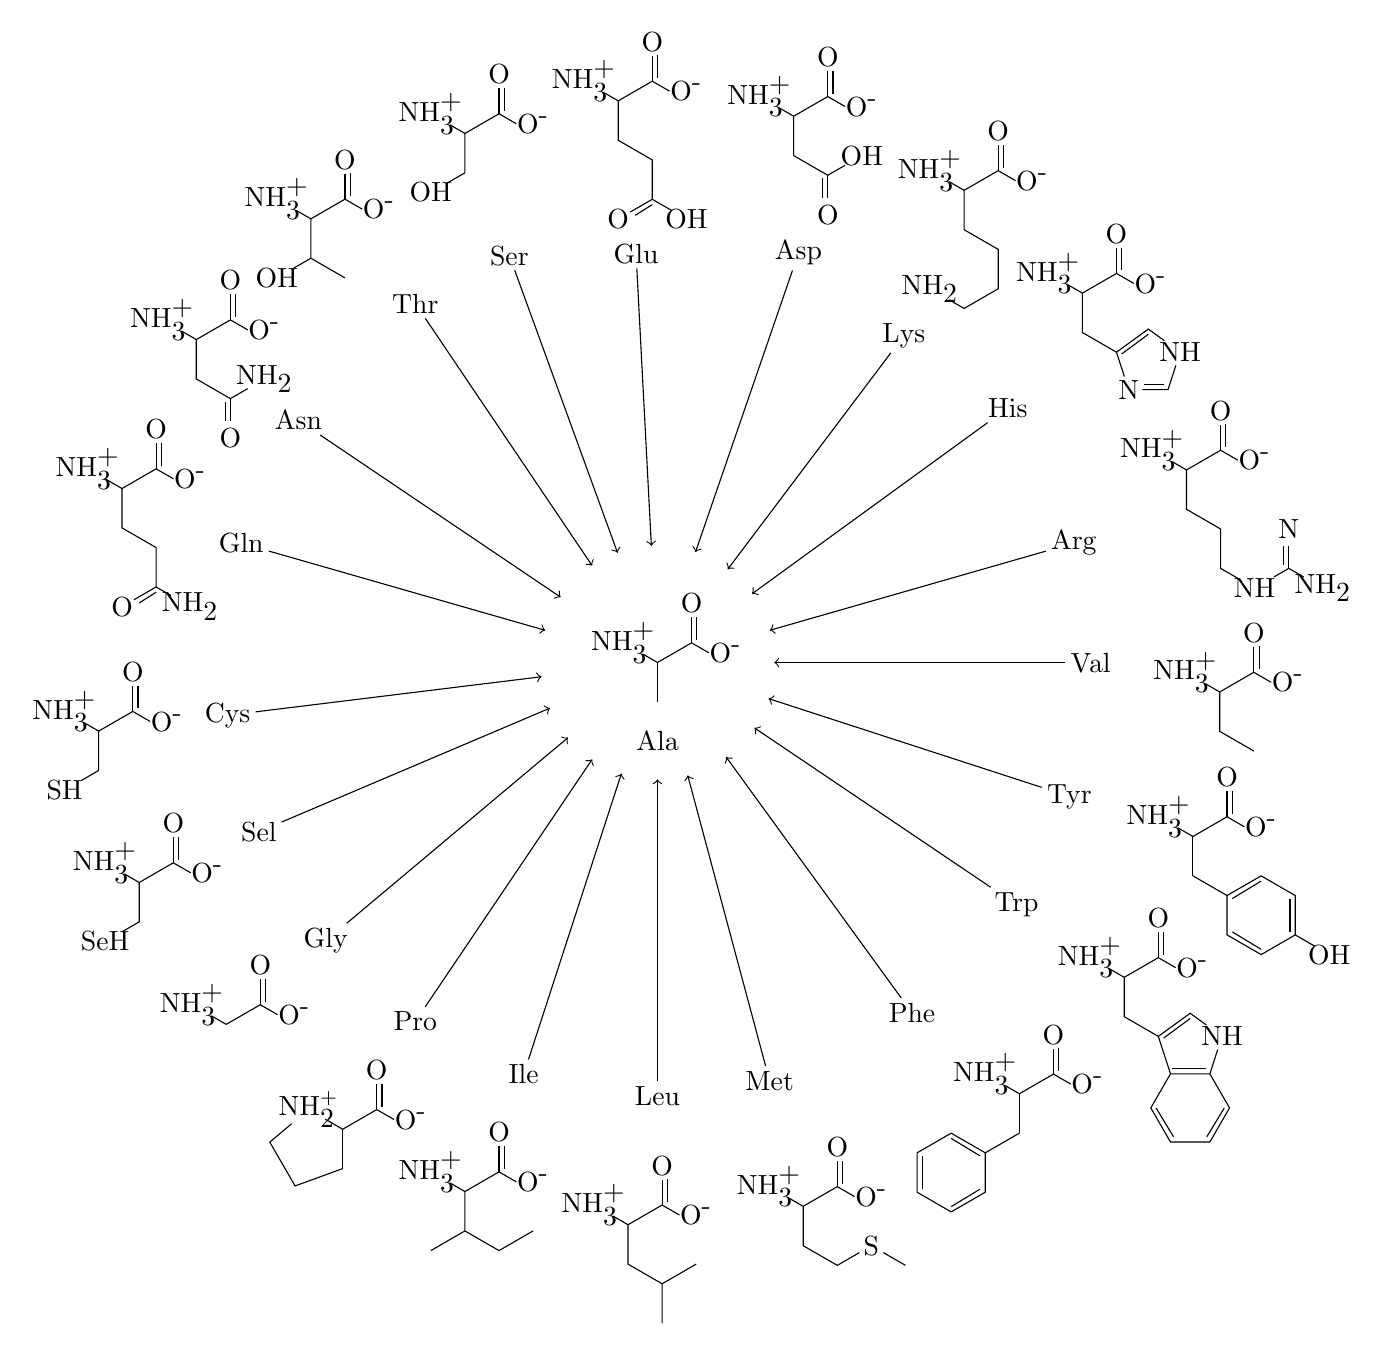
\begin{tikzpicture}
	\tikzstyle{every node}=[inner sep=1.7pt,anchor=center]
	%	to_x and from_x styles denote bonds terminating or starting in labeled nodes. x denotes the number of letters in the node label.
	\tikzstyle{to_1}=[shorten >=5pt]
	\tikzstyle{to_1i}=[shorten >=6pt]
	\tikzstyle{to_2}=[shorten >=7pt]
	\tikzstyle{to_3}=[shorten >=8pt]
	\tikzstyle{from_1}=[shorten <=5pt]
	\tikzstyle{from_1i}=[shorten <=6pt]
	\tikzstyle{from_2}=[shorten <=8pt]
	\def \ang {360.0/20}
	
	\Arginine{2+1*\ang:14.3}
	\node (Arg) at (-2+1*\ang:5.5) {Arg};
	\Histidine{5+2*\ang:14.3}
	\node (His) at (0+2*\ang:5.5) {His};
	\Lysine{3+3*\ang:14.3}
	\node (Lys) at (-1+3*\ang:5.2) {Lys};
	
	
	\AsparticAcid{4+4*\ang:14.3}
	\node (Asp) at (-1+4*\ang:5.5) {Asp};
	\GlutamicAcid{4+5*\ang:14.3}
	\node (Glu) at (3+5*\ang:5.2) {Glu};
	
	\Serine{2+6*\ang:14.3}
	\node (Ser) at (2+6*\ang:5.5) {Ser};
	%\SerineT{2+6*\ang:14.3}
	%\node at (2+6*\ang:5.5) {Ser};
	\Threonine{2+7*\ang:14.3}
	\node (Thr) at (-2+7*\ang:5.5) {Thr};
	\Asparagine{1+8*\ang:14.3}
	\node (Asn) at (2+8*\ang:5.5) {Asn};
	\Glutamine{0+9*\ang:14.3}
	\node (Gln) at (2+9*\ang:5.5) {Gln};
	
	\Cysteine{7+10*\ang:14.3}
	\node (Cys) at (7+10*\ang:5.5) {Cys};
	\Selenocysteine{5+11*\ang:14.3}
	\node (Sel) at (5+11*\ang:5.5) {Sel};
	\Glycine{4+12*\ang:14.3}
	\node (Gly) at (4+12*\ang:5.5) {Gly};
	\Proline{2+13*\ang:14.3}
	\node (Pro) at (2+13*\ang:5.5) {Pro};
	
	\node[draw, circle,minimum size=7pc, white] (Ala) at(0,0) {};
	\Alanine{0, 0}
	\node  at (0,-1) {Ala};
	
	\Isoleucine{-2+14*\ang:14.3}
	\node (Ile) at (0+14*\ang:5.5) {Ile};
	%\LeucineT{0+15*\ang:14.3}
	\Leucine{-3+15*\ang:14.3}
	\node (Leu) at (0+15*\ang:5.5) {Leu};
	
	\Methionine{-3+16*\ang:14.3}
	\node (Met) at (-3+16*\ang:5.5) {Met};
	\Phenylalanine{4+17*\ang:14.3}
	\node (Phe) at (0+17*\ang:5.5) {Phe};
	
	
	\Tryptophane{2+18*\ang:14.3}
	\node (Trp) at (2+18*\ang:5.5) {Trp};
	
	\Tyrosine{0+19*\ang:14.3}
	\node  (Tyr) at (0+19*\ang:5.5) {Tyr};
	\Valine{-3+20*\ang:14.3}
	\node (Val) at (0+20*\ang:5.5) {Val};
	
	\draw[->] (Arg) -- (Ala);
	\draw[->] (His) -- (Ala);
	\draw[->] (Lys) -- (Ala);
	\draw[->] (Asp) -- (Ala);
	\draw[->] (Glu) -- (Ala);
	\draw[->] (Ser) -- (Ala);
	\draw[->] (Thr) -- (Ala);
	\draw[->] (Asn) -- (Ala);
	\draw[->] (Gln) -- (Ala);
	\draw[->] (Cys) -- (Ala);
	\draw[->] (Sel) -- (Ala);
	\draw[->] (Gly) -- (Ala);
	\draw[->] (Pro) -- (Ala);
	\draw[->] (Ile) -- (Ala);
	\draw[->] (Leu) -- (Ala);
	\draw[->] (Met) -- (Ala);
	\draw[->] (Phe) -- (Ala);
	\draw[->] (Trp) -- (Ala);
	\draw[->] (Tyr) -- (Ala);
	\draw[->] (Val) -- (Ala);
	\end{tikzpicture}
}

